  % Documentación de la aplicación — Etapa 2
% Compilar desde esta carpeta:  latexmk -pdf aplicacion.tex
\documentclass[11pt,a4paper]{article}

% ------------------------------------------------------------------ paquetes
\usepackage[utf8]{inputenc}
\usepackage[T1]{fontenc}
\usepackage{lmodern}
\usepackage{textcomp}
\usepackage[spanish,es-tabla,es-noshorthands]{babel}
\usepackage[margin=2.5cm]{geometry}
\usepackage{microtype}
\usepackage{graphicx}
\usepackage{float}
\usepackage{booktabs}
\usepackage{tabularx}
\usepackage{longtable}
\usepackage{array}
\usepackage{enumitem}
\usepackage[table]{xcolor}
\usepackage{listings}
\usepackage{upquote}
\usepackage{caption}
\usepackage{tikz}
\usetikzlibrary{arrows.meta,positioning}
\usepackage{underscore}
\usepackage[hyphens]{url}
\usepackage[hidelinks]{hyperref}

\graphicspath{{../img/}}
\captionsetup{font=small,labelfont=bf}
\setlist{itemsep=2pt,topsep=4pt}
\renewcommand{\arraystretch}{1.25}
\newcolumntype{Y}{>{\raggedright\arraybackslash}X}

% Código: fondo gris claro, sin numeración, con acentos y símbolos en UTF-8
\definecolor{fondocodigo}{gray}{0.95}
\lstset{
  basicstyle=\ttfamily\small,
  backgroundcolor=\color{fondocodigo},
  frame=none,
  breaklines=true,
  breakatwhitespace=false,
  columns=fullflexible,
  keepspaces=true,
  showstringspaces=false,
  xleftmargin=6pt, xrightmargin=6pt,
  aboveskip=8pt, belowskip=8pt,
  literate=
    {á}{{\'a}}1 {é}{{\'e}}1 {í}{{\'i}}1 {ó}{{\'o}}1 {ú}{{\'u}}1
    {Á}{{\'A}}1 {É}{{\'E}}1 {Í}{{\'I}}1 {Ó}{{\'O}}1 {Ú}{{\'U}}1
    {ñ}{{\~n}}1 {Ñ}{{\~N}}1 {ü}{{\"u}}1
    {«}{{\guillemotleft}}1 {»}{{\guillemotright}}1
    {←}{{$\leftarrow$}}1 {–}{{--}}1
}
\newcommand{\cod}[1]{\texttt{#1}}
% Título + bloque de código que no se separan entre páginas
\newenvironment{bloque}[1]%
  {\par\medskip\noindent\begin{minipage}{\linewidth}#1}%
  {\end{minipage}\par\medskip}
% Rutas y URL largas: se pueden cortar en / . - para no salirse del margen
\urlstyle{tt}
\newcommand{\ruta}[1]{\path{#1}}

% ================================================================= documento
\begin{document}

\begin{titlepage}
    \centering
    \rule{\linewidth}{1pt}\\[0.5cm]
    {\LARGE\bfseries Instituto Tecnológico de Costa Rica}\\[0.5cm]
    \rule{\linewidth}{1pt}\\[1.5cm]
    \rule{0.7\linewidth}{0.4pt}\\[1cm]
    {\Large\textsc{Proyecto 2}}\\[1.5cm]
    \begin{minipage}{0.7\textwidth}
        \centering
        {\large\textbf{Integrantes:}\\[0.3cm]
        {\large Fabián Agüero, Jafeth Pérez}}
    \end{minipage}\\[1.5cm]
    {\large\today}\\[0.5cm]
    \rule{\linewidth}{1pt}
    \vfill
\end{titlepage}


\tableofcontents
\newpage

% ---------------------------------------------------------------------------
\section{Tecnologías utilizadas}

\begin{table}[H]
\centering\small
\begin{tabularx}{\textwidth}{@{}lllY@{}}
\toprule
\textbf{Capa} & \textbf{Tecnología} & \textbf{Versión} & \textbf{Para qué se usa} \\
\midrule
Motor de búsqueda & Apache Solr (imagen oficial de Docker) & 9.7 & Índice, consultas, facets y filtros espaciales \\
Geometría & JTS Topology Suite (\cod{jts-core}) & 1.19.0 & Permite que Solr acepte polígonos arbitrarios (WKT) \\
Contenedores & Docker Compose & --- & Levanta Solr con el core \cod{insectos} y la librería JTS \\
Backend & Python, FastAPI, Uvicorn & 3.12 / 0.115 / 0.34 & API REST entre la interfaz y Solr \\
Cliente HTTP & httpx & 0.28 & Envío de consultas a Solr \\
Pruebas & pytest & 8.3 & 22 pruebas automáticas contra el Solr real \\
Frontend & React, Vite & 18.3 / 5.4 & Interfaz gráfica de una sola página \\
Mapa & Leaflet, react-leaflet (OpenStreetMap) & 1.9 / 4.2 & Mapa interactivo, puntos y dibujo de polígonos \\
Gráficos & Recharts & 2.13 & Barras, histogramas, barras apiladas \\
\bottomrule
\end{tabularx}
\caption{Tecnologías de la aplicación.}
\end{table}

\paragraph{Por qué estas tecnologías.}
\begin{itemize}
  \item \textbf{FastAPI} valida automáticamente los datos que llegan de la interfaz
        (por ejemplo, que la latitud esté entre $-90$ y $90$) y genera documentación
        interactiva en \cod{/docs}.
  \item \textbf{React} permite armar los formularios a partir de una descripción de cada
        consulta, sin escribir una pantalla por consulta.
  \item \textbf{Leaflet} es liviano y usa renderizado en \emph{canvas}, lo que permite
        dibujar miles de puntos sin que el mapa se vuelva lento.
\end{itemize}

% ---------------------------------------------------------------------------
\section{Arquitectura y comunicación con Apache Solr}

\begin{figure}[H]
\centering
\begin{tikzpicture}[
  caja/.style={draw, rounded corners=3pt, align=left, inner sep=7pt, font=\small, minimum height=2.6cm},
  flecha/.style={-{Stealth[length=2.5mm]}, thick},
  etiqueta/.style={font=\footnotesize, fill=white, inner sep=1pt}]
  \node[caja, text width=3.3cm] (web) {\textbf{Navegador (React)}\\[3pt]
        · Consultas\\ · Mapa (Leaflet)};
  \node[caja, text width=4.6cm, right=1.6cm of web] (api) {\textbf{API FastAPI (Python)}\\[3pt]
        · \cod{main.py}: rutas\\ · \cod{consultas/}: arma los\\ \phantom{· }parámetros de Solr\\
        · \cod{solr.py}: envía y normaliza};
  \node[caja, text width=3.0cm, right=1.6cm of api] (solr) {\textbf{Apache Solr}\\[3pt]
        core \cod{insectos}\\ \cod{/select}};
  \draw[flecha] ([yshift=6mm]web.east) -- node[etiqueta, above=1pt]{JSON} ([yshift=6mm]api.west);
  \draw[flecha] ([yshift=-6mm]api.west) -- node[etiqueta, below=1pt]{JSON} ([yshift=-6mm]web.east);
  \draw[flecha] ([yshift=6mm]api.east) -- node[etiqueta, above=1pt]{HTTP} ([yshift=6mm]solr.west);
  \draw[flecha] ([yshift=-6mm]solr.west) -- node[etiqueta, below=1pt]{JSON} ([yshift=-6mm]api.east);
\end{tikzpicture}
\caption{Arquitectura: la interfaz nunca habla directamente con Solr; lo hace a través de la API.}
\end{figure}

\subsection{Flujo de una consulta (ejemplo: consulta 2)}

\begin{enumerate}
  \item \textbf{Formulario.} Al abrir la aplicación, la interfaz pide:
    \begin{itemize}
      \item \cod{GET /api/catalogo}: la descripción de las 13 consultas (campos del
            formulario, valores por defecto, tipo de gráfico), definida en
            \cod{backend/app/catalogo.py}.
      \item \cod{GET /api/opciones}: los valores reales de los menús (órdenes, provincias,
            áreas\ldots). La API los obtiene con un \emph{field facet} a Solr, así los menús
            solo ofrecen valores que existen en el índice.
    \end{itemize}
  \item \textbf{Envío.} Al ejecutar, la interfaz manda lo que eligió el usuario:
\begin{lstlisting}
POST /api/consultas/2
{"parametros": {"orden": "Lepidoptera",
                "categorias": ["Parque Nacional", "Reserva Biológica"],
                "excluir_provincia": "Limón"},
 "pagina": 0, "filas": 20}
\end{lstlisting}
  \item \textbf{Construcción.} La API llama a la función de esa consulta
        (\ruta{backend/app/consultas/convencionales.py} o \cod{geoespaciales.py}). Cada
        función recibe los valores del formulario y \textbf{devuelve un diccionario con los
        parámetros de Solr}:
\begin{lstlisting}
{"q": '(orden:"Lepidoptera" AND categoria_manejo:("Parque Nacional"
       OR "Reserva Biológica")) NOT provincia:"Limón"'}
\end{lstlisting}
        La API agrega la paginación (\cod{rows}, \cod{start}).
  \item \textbf{Ejecución.} \cod{backend/app/solr.py} envía los parámetros a
        \ruta{http://localhost:8983/solr/insectos/select} por \cod{POST} con
        \ruta{application/x-www-form-urlencoded}. Se usa POST para que los polígonos con
        muchos vértices no excedan el largo máximo de una URL.
  \item \textbf{Normalización.} Solr responde con estructuras distintas según el tipo de
        facet (\cod{facet_fields}, \cod{facet_ranges}, \cod{facet_queries}, \cod{facets} de
        la JSON Facet API\ldots). \cod{solr.py} las convierte a un formato único:
\begin{lstlisting}
{"numFound": 16076, "docs": [...], "qtime": 3,
 "facets": [{"nombre": "...", "tipo": "campo|rango|consulta|json",
             "buckets": [{"valor": "...", "conteo": 0,
                          "metricas": {}, "hijos": []}]}],
 "solr_params": {...},
 "solr_url": "http://localhost:8983/solr/insectos/select?..."}
\end{lstlisting}
  \item \textbf{Visualización.} La interfaz muestra el total, la tabla paginada, el
        gráfico del facet y el panel \textbf{«Consulta enviada a Solr»}, con los
        parámetros exactos y la URL equivalente. Esa URL se puede pegar en el navegador y
        Solr devuelve el mismo resultado.
\end{enumerate}

\begin{figure}[H]
\centering
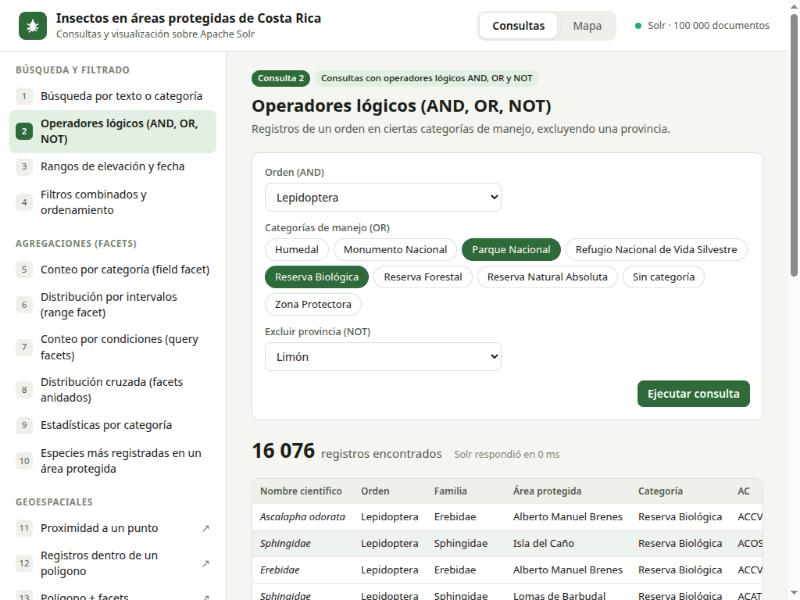
\includegraphics[width=0.85\textwidth]{02-operadores-logicos.jpg}
\caption{Consulta 2: formulario y resultado.}
\end{figure}

\begin{figure}[H]
\centering
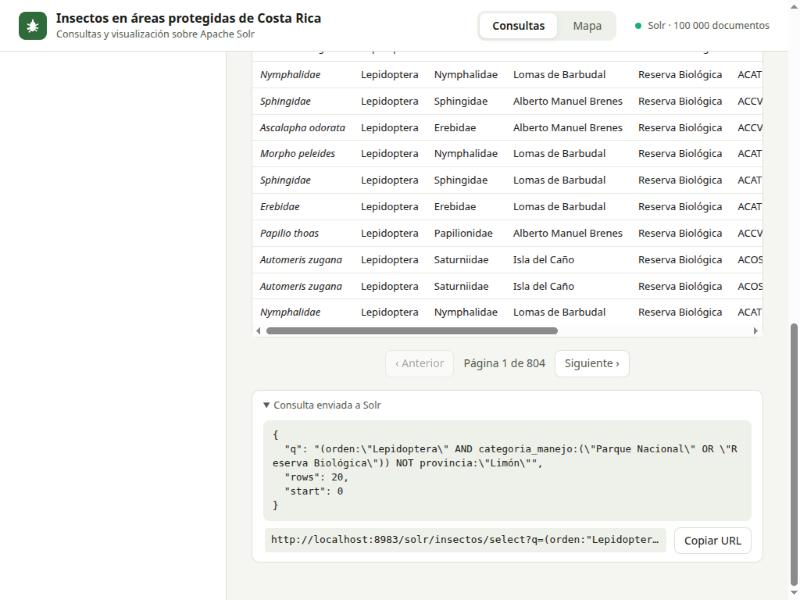
\includegraphics[width=0.85\textwidth]{02-consulta-enviada-a-solr.jpg}
\caption{Panel «Consulta enviada a Solr» de la consulta 2.}
\end{figure}

\subsection{Rutas de la API}

\begin{table}[H]
\centering\small
\begin{tabularx}{\textwidth}{@{}lY@{}}
\toprule
\textbf{Método y ruta} & \textbf{Descripción} \\
\midrule
\cod{GET /api/estado} & Conexión con Solr y cantidad de documentos (indicador del encabezado) \\
\cod{GET /api/catalogo} & Consultas disponibles y sus formularios \\
\cod{GET /api/opciones} & Valores de los menús desplegables \\
\cod{POST /api/consultas/\{1..10\}} & Ejecuta una consulta convencional \\
\cod{GET /api/mapa/puntos} & Muestra aleatoria de puntos para el modo «Explorar» del mapa \\
\cod{POST /api/geo/proximidad} & Consulta 11 \\
\cod{POST /api/geo/poligono} & Consulta 12 \\
\cod{POST /api/geo/poligono-facets} & Consulta 13 \\
\bottomrule
\end{tabularx}
\caption{Rutas de la API REST.}
\end{table}

Si Solr devuelve un error (por ejemplo, de sintaxis), la API responde con el mismo código
HTTP y el mensaje de Solr, y la interfaz lo muestra junto con la consulta que lo causó.

% ---------------------------------------------------------------------------
\section{Configuración e indexación en Solr}

\subsection{Contenedor}

\cod{docker-compose.yml} levanta un único nodo de Solr 9.7:
\begin{itemize}
  \item Se construye desde \ruta{solr/Dockerfile}, que parte de \cod{solr:9.7} y descarga
        \ruta{jts-core-1.19.0.jar} de Maven Central a
        \ruta{/opt/solr/server/solr-webapp/webapp/WEB-INF/lib/}. La imagen oficial no trae
        JTS, y sin esa librería Solr no puede crear el campo espacial.
  \item \cod{solr-precreate insectos} crea el core al arrancar.
  \item El puerto 8983 se publica solo en \cod{127.0.0.1}.
  \item El volumen \cod{solr_data} (\cod{/var/solr}) conserva el índice entre reinicios.
\end{itemize}

\subsection{Esquema}

\cod{solr/crear_esquema.py} define el esquema mediante la \textbf{Schema API}. Desactiva
la creación automática de campos (\cod{update.autoCreateFields=false}) y agrega cada campo
con su tipo. Un documento corresponde a una ocurrencia de insecto ya unida con su área
protegida.

\begin{table}[H]
\centering\small
\begin{tabularx}{\textwidth}{@{}YlY@{}}
\toprule
\textbf{Campo} & \textbf{Tipo} & \textbf{Uso en las consultas} \\
\midrule
\cod{nombre_cientifico}, \cod{localidad} & \cod{text_general} (analizado) & Búsqueda por palabras (consulta 1) \\
\cod{texto} (por \cod{copyField} de nombre, orden, familia, localidad, área y categoría) & \cod{text_es} & Búsqueda general en español \\
\cod{orden}, \cod{familia}, \cod{genero}, \cod{especie}, \cod{provincia}, \cod{area_protegida}, \cod{categoria_manejo}, \cod{area_conservacion}, \cod{estacion}, \cod{piso_altitudinal}, \ldots & \cod{string} (docValues) & Filtros exactos y facets \\
\cod{elevacion_m}, \cod{latitud}, \cod{longitud}, \cod{area_protegida_km2} & \cod{pdouble} & Rangos, estadísticas \\
\cod{anio}, \cod{mes} & \cod{pint} & Range facet por año \\
\cod{fecha_evento} & \cod{pdate} & Rangos temporales y orden \\
\cod{dentro_asp} & \cod{boolean} & Query facets \\
\textbf{\cod{ubicacion}} & \textbf{\cod{ubicacion_rpt}} & Consultas geoespaciales \\
\bottomrule
\end{tabularx}
\caption{Campos principales del esquema.}
\end{table}

El tipo \textbf{\cod{ubicacion_rpt}} es un \cod{SpatialRecursivePrefixTreeFieldType} con:
\begin{itemize}
  \item \cod{spatialContextFactory=JTS}: acepta polígonos arbitrarios en formato WKT, no
        solo rectángulos ni círculos.
  \item \cod{geo=true} y \cod{distanceUnits=kilometers}: coordenadas geográficas y
        distancias en km.
  \item \cod{distErrPct=0}: precisión exacta en los bordes. Con el valor por defecto
        (0,025), Solr aproxima la forma del polígono y llegaba a incluir puntos que estaban
        justo afuera.
  \item \cod{validationRule=repairBuffer0}: repara polígonos inválidos, como uno dibujado
        con lados que se cruzan.
\end{itemize}

\subsection{Indexación}

\cod{solr/indexar.py} lee el archivo JSONL o CSV que produce Spark y lo envía en lotes de
5\,000 documentos a \cod{/update}, con un \emph{commit} al final. Si el campo
\cod{ubicacion} no viene, lo construye como \cod{"lat,lon"}. Los 100\,000 documentos de
prueba se indexan en unos 7~s.

% ---------------------------------------------------------------------------
\section{Las consultas y cómo apoyan el objetivo del proyecto}

El objetivo es \textbf{analizar la población de insectos en las áreas silvestres
protegidas (ASP)}. Para eso las consultas responden tres tipos de preguntas:
\emph{¿dónde?} (áreas, regiones, cercanía), \emph{¿qué?} (qué órdenes y especies) y
\emph{¿en qué condiciones?} (elevación, época, estación).

En cada tabla, \textbf{«Resultado»} es lo que devolvió Solr con los valores por defecto
del formulario y los datos de prueba. Debajo de cada tabla están los parámetros exactos
que la aplicación envía a Solr.

\subsection{Búsqueda y filtrado}

\begin{table}[H]
\centering\small
\begin{tabularx}{\textwidth}{@{}cp{3.6cm}Yl@{}}
\toprule
\textbf{\#} & \textbf{Requisito} & \textbf{Pregunta que responde} & \textbf{Resultado} \\
\midrule
1 & Búsqueda por campos textuales o categóricos & ¿Dónde se ha registrado un taxón? ¿Qué hay registrado en un área? & 1\,204 / 2\,928 \\
2 & Operadores AND, OR y NOT & ¿Cuántas mariposas hay en las categorías de protección más estrictas, fuera del Caribe? & 16\,076 \\
3 & Rangos numéricos y temporales & ¿Qué se colectó en zonas de montaña durante un periodo? & 11\,968 \\
4 & Combinación de filtros y ordenamiento por varios atributos & Registros más recientes de escarabajos en el Área de Conservación Osa & 2\,935 \\
\bottomrule
\end{tabularx}
\caption{Consultas de búsqueda y filtrado.}
\end{table}

\begin{bloque}{\textbf{Consulta 1} (texto general «Morpho» / área protegida «Volcán Poás»):}
\begin{lstlisting}
q=Morpho   defType=edismax   qf=texto   q.op=AND
q=*:*      fq=area_protegida:"Volcán Poás"
\end{lstlisting}
\end{bloque}

\begin{bloque}{\textbf{Consulta 2:}}
\begin{lstlisting}
q=(orden:"Lepidoptera"
   AND categoria_manejo:("Parque Nacional" OR "Reserva Biológica"))
  NOT provincia:"Limón"
\end{lstlisting}
\end{bloque}

\begin{bloque}{\textbf{Consulta 3:}}
\begin{lstlisting}
q=*:*
fq=elevacion_m:[1000 TO 2500]
fq=fecha_evento:[1995-01-01T00:00:00Z TO 2005-12-31T23:59:59.999Z]
\end{lstlisting}
\end{bloque}

\begin{bloque}{\textbf{Consulta 4:}}
\begin{lstlisting}
q=*:*
fq=orden:"Coleoptera"
fq=area_conservacion:"ACOSA"
sort=fecha_evento desc, elevacion_m asc, id asc
\end{lstlisting}
\end{bloque}

\paragraph{Decisiones de diseño.}
\begin{itemize}
  \item En la consulta 2 la expresión va completa en \cod{q} para que los tres operadores
        se vean en una sola expresión booleana.
  \item En la 3 y la 4 cada condición es un \cod{fq} aparte: son filtros de sí/no que no
        afectan la relevancia, y Solr guarda cada uno en caché por separado.
  \item Un filtro opcional que se deja vacío no restringe la búsqueda.
  \item Los valores elegidos por el usuario se ponen entre comillas y se escapan.
  \item Los nombres de campo y de orden se validan contra una lista de permitidos, para
        que nadie pueda inyectar sintaxis de Solr.
\end{itemize}

\subsection{Facets}

\begin{table}[H]
\centering\small
\begin{tabularx}{\textwidth}{@{}cp{3.2cm}Yp{4.2cm}@{}}
\toprule
\textbf{\#} & \textbf{Requisito} & \textbf{Pregunta que responde} & \textbf{Resultado} \\
\midrule
5 & Field facet & ¿Qué órdenes dominan los registros? (también por área, provincia, categoría\ldots) & Lepidoptera 29\,909, Coleoptera 25\,010, Hymenoptera 17\,997\ldots \\
6 & Range facet & ¿Cómo se distribuyen los registros según la elevación, o según el año? & $[0, 250)$: 46\,645; $[250, 500)$: 11\,459\ldots \\
7 & Query facets & ¿Cuántos registros hay por piso altitudinal, dentro o fuera de un ASP y por estación? & Basal 58\,104, Premontano 25\,459, Montano bajo 8\,966\ldots \\
8 & Facets anidados & ¿Qué órdenes predominan en cada área de conservación? & ACC 16\,931 (5 órdenes)\ldots \\
9 & Facets con funciones estadísticas & Perfil altitudinal y riqueza de especies de cada área & Volcán Poás: 2\,928 registros, de 1\,516 a 3\,655~m, promedio 2\,401~m \\
10 & Field facet filtrado + estadísticas & ¿Cuáles son las especies más registradas en un área protegida? & Corcovado: 2\,841; \emph{Polybia occidentalis} 108, \emph{Calosoma sayi} 95\ldots \\
\bottomrule
\end{tabularx}
\caption{Consultas con facets.}
\end{table}

\begin{bloque}{\textbf{Consulta 5:}}
\begin{lstlisting}
q=*:*  rows=0  facet=true
facet.field=orden  facet.limit=10  facet.mincount=1  facet.sort=count
\end{lstlisting}
\end{bloque}

\begin{bloque}{\textbf{Consulta 6:}}
\begin{lstlisting}
q=*:*  rows=0  facet=true
facet.range=elevacion_m  facet.range.start=0  facet.range.end=3500
facet.range.gap=250  facet.mincount=0  facet.range.other=all
\end{lstlisting}
\end{bloque}

\begin{bloque}{\textbf{Consulta 7} (8 condiciones; se muestran algunas):}
\begin{lstlisting}
q=*:*  rows=0  facet=true
facet.query={!key='Piso basal (< 500 m)'}elevacion_m:[* TO 500}
facet.query={!key='Piso premontano (500–1500 m)'}elevacion_m:[500 TO 1500}
facet.query={!key='Dentro de un ASP'}dentro_asp:true
facet.query={!key='Estación seca (dic–abr)'}estacion:"Seca"
...
\end{lstlisting}
\end{bloque}

\begin{bloque}{\textbf{Consulta 8} (JSON Facet API):}
\begin{lstlisting}
q=*:*  rows=0
json.facet={"area_conservacion": {"type": "terms", "field": "area_conservacion",
              "limit": 12, "sort": "count desc",
              "facet": {"orden": {"type": "terms", "field": "orden",
                                  "limit": 5, "sort": "count desc"}}}}
\end{lstlisting}
\end{bloque}

\begin{bloque}{\textbf{Consulta 9:}}
\begin{lstlisting}
q=*:*  rows=0
json.facet={"area_protegida": {"type": "terms", "field": "area_protegida",
              "limit": 15, "sort": "count desc",
              "facet": {"elev_promedio": "avg(elevacion_m)",
                        "elev_min": "min(elevacion_m)",
                        "elev_max": "max(elevacion_m)",
                        "especies_distintas": "unique(especie)"}}}
\end{lstlisting}
\end{bloque}

\begin{bloque}{\textbf{Consulta 10:}}
\begin{lstlisting}
q=*:*  rows=0  fq=area_protegida:"Corcovado"
json.facet={"especies": {"type": "terms", "field": "especie", "limit": 10,
                         "sort": "count desc",
                         "facet": {"elev_promedio": "avg(elevacion_m)"}},
            "elev_promedio": "avg(elevacion_m)", "elev_min": "min(elevacion_m)",
            "elev_max": "max(elevacion_m)", "especies_distintas": "unique(especie)"}
\end{lstlisting}
\end{bloque}

\paragraph{Decisiones de diseño.}
\begin{itemize}
  \item En la consulta 7, los rangos de elevación usan \cod{\}} (extremo exclusivo) para
        que ningún registro caiga en dos pisos.
  \item Para la consulta 8 se eligió la \textbf{JSON Facet API} en lugar de
        \cod{facet.pivot} porque permite un límite distinto en cada nivel. Además es la
        misma API que se usa para las métricas de la 9 y la 10.
  \item La consulta 10 cuenta sobre \cod{especie}, así que solo incluye los registros
        identificados hasta especie. Los identificados solo hasta género o familia no
        entran en el ranking.
\end{itemize}

\begin{figure}[H]
\centering
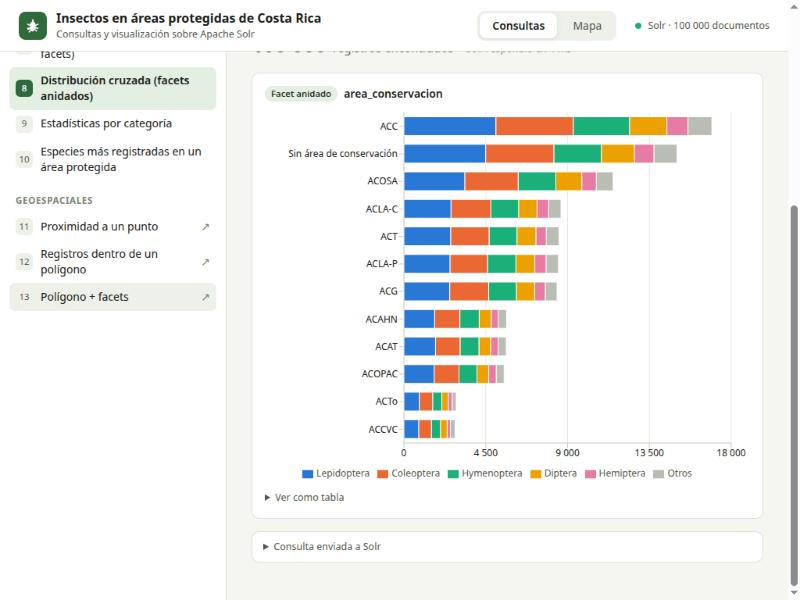
\includegraphics[width=0.85\textwidth]{08-facets-anidados.jpg}
\caption{Consulta 8: facets anidados (barras apiladas).}
\end{figure}

\begin{figure}[H]
\centering
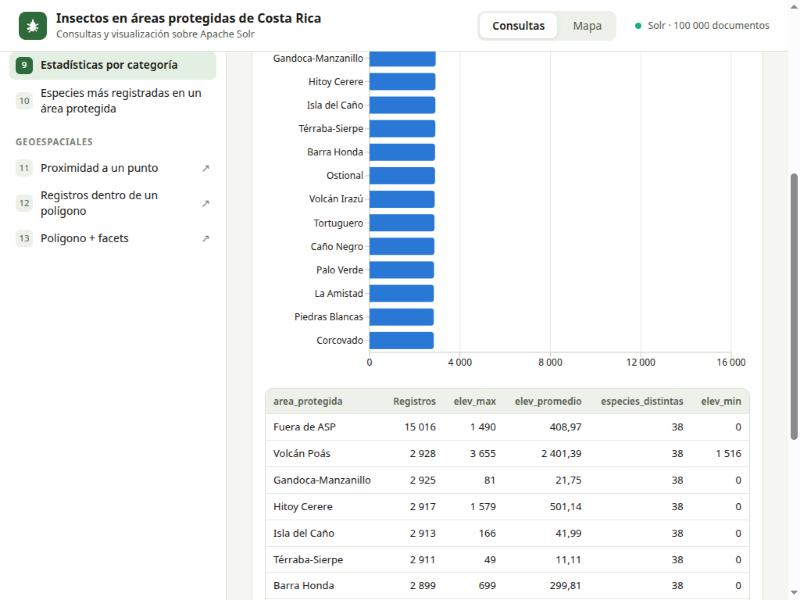
\includegraphics[width=0.85\textwidth]{09-estadisticas.jpg}
\caption{Consulta 9: estadísticas por área protegida.}
\end{figure}

\subsection{Geoespaciales}

\begin{table}[H]
\centering\small
\begin{tabularx}{\textwidth}{@{}cp{3.6cm}Yp{3.4cm}@{}}
\toprule
\textbf{\#} & \textbf{Requisito} & \textbf{Pregunta que responde} & \textbf{Resultado} \\
\midrule
11 & Proximidad con radio del usuario (+ filtro por atributo) & ¿Qué se ha registrado cerca de un punto, como una estación biológica o un sendero? & 1\,951 (579 Lepidoptera) \\
12 & Registros dentro de una región dibujada & ¿Qué hay en una región que no coincide con los límites administrativos, como un corredor biológico? & 2\,912 (península de Osa) \\
13 & Polígono combinado con facets & ¿Cómo se compone la población de insectos dentro de esa región? & Lepidoptera 848, Coleoptera 747, Hymenoptera 532\ldots \\
\bottomrule
\end{tabularx}
\caption{Consultas geoespaciales.}
\end{table}

\begin{bloque}{\textbf{Consulta 11} (San José, radio de 15~km; la última línea solo si se elige un orden):}
\begin{lstlisting}
q=*:*  sfield=ubicacion  pt=9.93,-84.08  d=15
fq={!geofilt}
sort=geodist() asc
fl=id,latitud,longitud,...,dist:geodist()
fq=orden:"Lepidoptera"
\end{lstlisting}
\end{bloque}

\begin{bloque}{\textbf{Consulta 12} (península de Osa, 5 vértices):}
\begin{lstlisting}
q=*:*
fq=ubicacion:"Intersects(POLYGON((-83.75 8.75, -83.3 8.7, -83.25 8.45,
                                  -83.55 8.35, -83.8 8.5, -83.75 8.75)))"
\end{lstlisting}
\end{bloque}

\begin{bloque}{\textbf{Consulta 13:} el mismo \cod{fq} de la consulta 12, más:}
\begin{lstlisting}
facet=true  facet.field=orden  facet.mincount=1  facet.limit=-1  facet.sort=count
\end{lstlisting}
\end{bloque}

\begin{figure}[H]
\centering
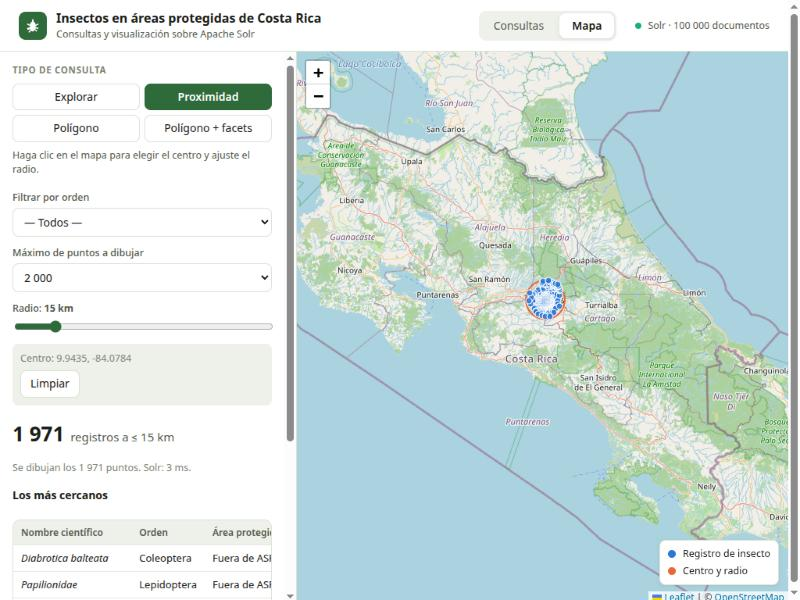
\includegraphics[width=0.85\textwidth]{11-proximidad.jpg}
\caption{Consulta 11: proximidad a un punto con radio de 15~km.}
\end{figure}

% ---------------------------------------------------------------------------
\section{Consultas geoespaciales a partir del polígono dibujado}

El mapa (pestaña \textbf{Mapa}) tiene cuatro modos: \emph{Explorar}, \emph{Proximidad},
\emph{Polígono} y \emph{Polígono + facets}.

\subsection{Procedimiento}

\begin{enumerate}
  \item \textbf{Dibujo libre.} En el modo \emph{Polígono}, cada clic sobre el mapa agrega
        un vértice. No hay límite de vértices y el polígono puede ser irregular o cóncavo.
    \begin{itemize}
      \item \textbf{Deshacer} quita el último vértice.
      \item \textbf{Limpiar} empieza de nuevo.
      \item \textbf{Cerrar y consultar}, o un clic sobre el primer vértice, cierra el
            polígono.
    \end{itemize}
  \item \textbf{Envío.} La interfaz manda los vértices en el orden en que se dibujaron,
        como \cod{[lat, lon]} (el orden que usa Leaflet), junto con los filtros por
        atributo y el máximo de puntos a dibujar (vértices de ejemplo):
\begin{lstlisting}
POST /api/geo/poligono-facets
{"vertices": [[10.05,-84.40],[10.10,-83.95],[9.85,-83.85],
              [9.87,-84.08],[9.75,-84.25]],
 "filtros": {"orden": "Lepidoptera"}, "filas": 2000, "campo_facet": "orden"}
\end{lstlisting}
        La API valida que haya al menos 3 vértices y que las coordenadas estén en rango.
  \item \textbf{Construcción del WKT.} La función \cod{poligono_wkt()} de
        \ruta{backend/app/consultas/geoespaciales.py}:
    \begin{itemize}
      \item invierte cada vértice a \textbf{\cod{lon lat}}, porque WKT usa el orden
            \emph{x y};
      \item quita el último vértice si es igual al primero, para no duplicarlo;
      \item exige al menos 3 vértices distintos;
      \item \textbf{cierra el anillo} repitiendo el primer vértice al final.
    \end{itemize}
        Resultado:
\begin{lstlisting}
POLYGON((-84.4 10.05, -83.95 10.1, -83.85 9.85, -84.08 9.87,
         -84.25 9.75, -84.4 10.05))
\end{lstlisting}
  \item \textbf{Filtro en Solr.} El polígono viaja dentro de un \cod{fq} sobre el campo RPT:
\begin{lstlisting}
fq=ubicacion:"Intersects(POLYGON((...)))"
fq=orden:"Lepidoptera"            ← condición sobre otro atributo (opcional)
facet.field=orden                 ← solo en el modo «Polígono + facets»
\end{lstlisting}
        Para puntos, \cod{Intersects} e \cod{IsWithin} dan el mismo resultado. Se usa
        \cod{Intersects} porque es la operación recomendada, es más barata e incluye los
        puntos sobre el borde. Solr resuelve el filtro con el índice espacial (árbol de
        prefijos) y la geometría de JTS.
  \item \textbf{Resultado.} La interfaz:
    \begin{itemize}
      \item borra los puntos anteriores y dibuja \textbf{solo los documentos que devolvió
            Solr};
      \item muestra el total \cod{numFound} («20\,757 registros dentro del polígono»),
            aunque se dibuje una cantidad menor de puntos;
      \item en el modo con facets, muestra debajo el gráfico de distribución por el campo
            elegido.
    \end{itemize}
\end{enumerate}

\paragraph{El filtrado lo hace Solr, no la aplicación.} El backend nunca pide todos los
registros para filtrarlos en Python: el polígono se envía dentro del \cod{fq}. Esto se
puede verificar en el panel «Consulta enviada a Solr», y una prueba automática
(sección~\ref{sec:pruebas}) comprueba que la consulta enviada contiene el \cod{POLYGON}.

\begin{figure}[H]
\centering
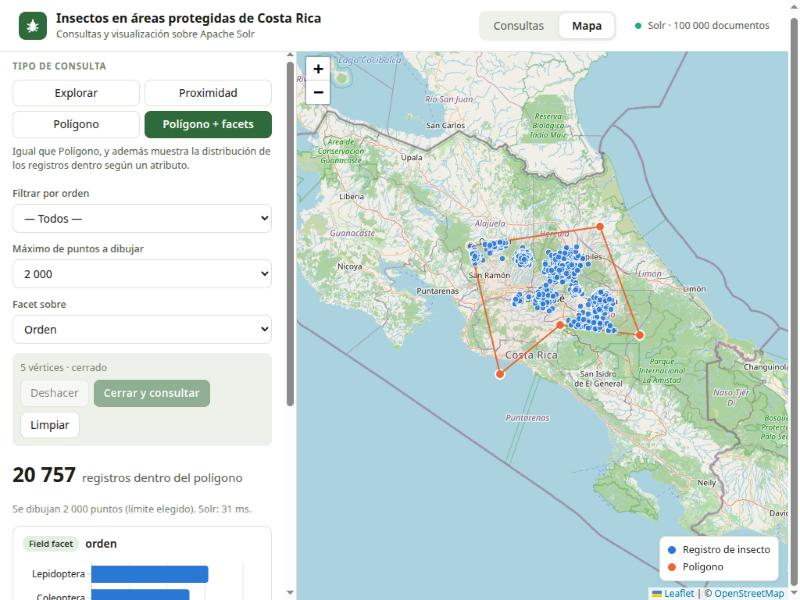
\includegraphics[width=0.85\textwidth]{13-poligono-facets.jpg}
\caption{Consulta 13: polígono cóncavo de 5 vértices con el facet por orden.}
\end{figure}

\subsection{Proximidad}

En el modo \emph{Proximidad}, un clic fija el centro y un deslizador elige el radio
(1--100~km). La consulta se repite sola 250~ms después de cada cambio. Los parámetros
compartidos \cod{sfield}, \cod{pt} y \cod{d} los usan a la vez tres partes de la consulta:
\begin{itemize}
  \item \cod{\{!geofilt\}}: el filtro por distancia;
  \item \cod{geodist()}: el orden, del más cercano al más lejano;
  \item el campo calculado \cod{dist}: la distancia de cada registro en km, que se muestra
        en la tabla.
\end{itemize}

% ---------------------------------------------------------------------------
\section{Pruebas realizadas y resultados}
\label{sec:pruebas}

\subsection{Pruebas automáticas}

Ubicadas en \cod{backend/tests/}. Se ejecutan contra el Solr real con:
\begin{lstlisting}
backend/.venv/bin/pytest backend/tests -v
\end{lstlisting}

Las pruebas \textbf{no comparan la consulta escrita}, sino que \textbf{el resultado tenga
sentido}. En las geoespaciales, la geometría se recalcula en Python de forma independiente
a Solr.

{\small
\begin{longtable}{@{}p{5.6cm}p{9.6cm}@{}}
\caption{Pruebas automáticas.}\\
\toprule
\textbf{Prueba} & \textbf{Qué verifica} \\
\midrule
\endfirsthead
\toprule
\textbf{Prueba} & \textbf{Qué verifica} \\
\midrule
\endhead
\bottomrule
\endfoot
\cod{test_consulta_1_*} (3) & Búsqueda general, coincidencia exacta y valores con espacios («Volcán Poás») \\
\cod{test_consulta_2_logicos} & Todo documento cumple el orden, alguna de las categorías y no está en la provincia excluida \\
\cod{test_consulta_3_rangos} & Todas las elevaciones y fechas están dentro de los rangos \\
\cod{test_consulta_4_filtros_y_orden} & Se cumplen los filtros y el orden (fecha desc, luego elevación asc) \\
\cod{test_consulta_4_filtros_vacios_no_filtran} & Con filtros vacíos, \cod{numFound} es igual al total del índice \\
\cod{test_consulta_5_field_facet} & Respeta el límite y ordena los buckets de mayor a menor \\
\cod{test_consulta_6_*} (2) & Los intervalos empiezan en 0, 500, 1000\ldots\ (7 buckets) y en 1985, 1990\ldots\ por año \\
\cod{test_consulta_7_query_facets} & Al menos 3 condiciones con conteo \\
\cod{test_consulta_8_anidado} & Cada bucket tiene un segundo nivel, respeta los límites y los hijos no superan al padre \\
\cod{test_consulta_9_estadisticas} & Cada grupo trae al menos 3 métricas \\
\cod{test_consulta_10_ranking} & Son especies (género + epíteto) y los conteos no superan el total del área \\
\cod{test_consulta_11_proximidad} & Distancia de Haversine de cada punto $\le$ radio, y resultados del más cercano al más lejano \\
\cod{test_consulta_11_con_filtro} & El filtro por orden reduce el resultado y todos los documentos son de ese orden \\
\cod{test_consulta_12_poligono} & Cada punto devuelto está dentro del polígono según \emph{ray casting} en Python, y la consulta enviada contiene \cod{POLYGON} \\
\cod{test_consulta_12_poligono_cerrado_o_no} & Enviar el polígono abierto o cerrado da el mismo total \\
\cod{test_consulta_13_poligono_facets} & La suma de los buckets es igual al total dentro del polígono \\
\cod{test_normalizacion.py} (3) & Conversión de parámetros y normalización de cada tipo de facet, sin necesitar Solr \\
\end{longtable}
}

\textbf{Resultado:} \cod{22 passed} (las 22 pruebas pasan).

\subsection{Pruebas manuales en la interfaz}

\begin{table}[H]
\centering\small
\begin{tabularx}{\textwidth}{@{}YY@{}}
\toprule
\textbf{Prueba} & \textbf{Resultado} \\
\midrule
Ejecutar las consultas 1--10 con los valores por defecto & Los totales coinciden con los de la sección 4; los gráficos se dibujan sin errores en la consola \\
Abrir directamente en Solr la URL del panel «Consulta enviada a Solr» (consulta 2) & Mismo \cod{numFound} (16\,076) \\
Dibujar un polígono cóncavo de 5 vértices sobre el Valle Central (modo polígono + facets) & 20\,757 registros, solo se dibujan puntos interiores, gráfico por orden \\
Proximidad con un clic cerca de San José, radio de 15~km & 1\,971 registros dentro del círculo, tabla con los más cercanos \\
Polígono con lados cruzados (forma de 8) & Solr lo repara (\cod{repairBuffer0}) y responde (4\,244 registros); no hay error \\
Reiniciar el contenedor (\cod{docker compose restart}) & El índice conserva los 100\,000 documentos \\
Ventanas de 1\,009~px y de 375~px (celular) & Sin desplazamiento horizontal de la página: las tablas anchas se desplazan dentro de su recuadro \\
\bottomrule
\end{tabularx}
\caption{Pruebas manuales.}
\end{table}

% ---------------------------------------------------------------------------
\section{Conclusiones}

\subsection{Conclusiones}

\begin{itemize}
  \item \textbf{Solr cubre todo el análisis.} Búsqueda, filtros, cinco tipos de facets,
        estadísticas y geometría se resuelven en el índice, con tiempos de respuesta de
        pocos milisegundos sobre 100\,000 documentos. La aplicación solo arma la consulta y
        presenta el resultado.
  \item \textbf{El campo espacial requiere configuración explícita.} Para consultar
        polígonos arbitrarios hacen falta tres cosas que no vienen por defecto: la
        librería JTS en la imagen, \cod{spatialContextFactory=JTS} y \cod{distErrPct=0}.
        Sin la última, el filtro aceptaba puntos fuera del borde del polígono.
  \item \textbf{Separar la construcción de la consulta de su ejecución} hizo posible probar
        cada consulta de forma aislada. Cada función solo devuelve parámetros, y el panel
        «Consulta enviada a Solr» hace visible qué se ejecuta en cada momento.
  \item \textbf{Para el objetivo del proyecto}, la combinación más útil es el polígono con
        facets (consulta 13). Permite delimitar una región que no coincide con los límites
        oficiales, como un corredor biológico o una cuenca, y ver de inmediato cómo se
        compone su población de insectos.
\end{itemize}

\end{document}
